\RequirePackage{tikz} 
\documentclass[sn-mathphys]{sn-jnl}

\jyear{2021}%

\theoremstyle{thmstyleone}%
\newtheorem{theorem}{Theorem}%  meant for continuous numbers
\newtheorem{proposition}[theorem]{Proposition}% 


\theoremstyle{thmstyletwo}%
\newtheorem{example}{Example}%
\newtheorem{remark}{Remark}%

\theoremstyle{thmstylethree}%
\newtheorem{definition}{Definition}%

\usepackage{subcaption}
\graphicspath{{images/}}
\usepackage{adjustbox}

\usepackage{accents}
% ---------- Standard Commands ------------------

\usepackage{color}
\newcommand\red[1]{{\textcolor{red}{#1}}}
\newcommand\blue[1]{{\textcolor{blue}{#1}}}

\newcommand{\DS}[1]{\red{DS: #1}}
\newcommand{\Sam}[1]{\blue{Sam: #1}}
% ---------- new variables ------------------
\newcommand{\Hinf}{$H_\infty$\xspace}
\newcommand{\photoa}{PH-A}
\newcommand{\photob}{PH-B}
\newcommand{\photodistance}{d}


% ---------- new commands ------------------
\newcommand{\vect}[1]{\bm{#1}}		% vectors
\newcommand{\matr}[1]{\bm{#1}}		% matrices
\newcommand{\nR}[1]{\mathbb{R}^{#1}}		% real number
\newcommand{\nT}[1]{\mathbb{T}^{#1}}		% real number
\newcommand{\define}{:=}			% define symbol
\newcommand{\modulus}[1]{\left| #1 \right|}	% abs
\newcommand{\matrice}[1]{\begin{bmatrix} #1 \end{bmatrix}}	% matrix
\newcommand{\smallmatrice}[1]{\left[\begin{smallmatrix} #1 \end{smallmatrix}\right]}	% matrix
\newcommand{\cosp}[1]{\cos \left( #1 \right)}	% cos with brace
\newcommand{\sinp}[1]{\sin \left( #1 \right)}	% sin with brace
\newcommand{\determinant}[1]{\text{det}\left(#1\right)} 	% determinant
\newcommand{\sgn}[1]{\text{sgn}\left( #1 \right)}			% signum
\newcommand{\atanTwo}[1]{{\rm atan2}\left( #1\right)}		% atan2
\newcommand{\acotTwo}[1]{{\rm acot2}\left( #1\right)}		% acot2
\newcommand{\upperRomannumeral}[1]{\uppercase\expandafter{\romannumeral#1}}	% roman numbers
\newcommand{\lowerromannumeral}[1]{\romannumeral#1\relax}
\newcommand{\vSpace}{\;\,}
\newcommand{\ubar}[1]{\underaccent{\bar}{#1}}

%-----------Functions------------------------
\newcommand{\minEig}[1]{\lambda_{\text{min}}[#1]}
\newcommand{\maxEig}[1]{\lambda_{\text{max}}[#1]}
\newcommand{\transp}{^\top}


% --------- References ----------------------
\newcommand{\fig}{Fig.~}	% figure ref
\newcommand{\eqn}{Eq.~}	% equation ref
\newcommand{\tab}{Tab.~}	% table ref
\newcommand{\cha}{Chap.~}	% chapter ref
\newcommand{\sect}{Sec.~}	% section ref
\newcommand{\alg}{Algorithm~}

% --------- Variables -----------------------

% General
\renewcommand{\frame}{\mathcal{F}}		% frame
\newcommand{\origin}{O}						% origin
\newcommand{\vX}{\vect{x}}					% x-axis
\newcommand{\vY}{\vect{y}}					% y-axis
\newcommand{\vZ}{\vect{z}}					% z-axis
\newcommand{\pos}{\vect{p}}				% position vector
\newcommand{\dpos}{\vect{v}}				% velocity vector
\newcommand{\rotMat}{\matr{R}}				% rotation matrix
\newcommand{\rotMatVectAngle}[2]{\rotMat_{#1}(#2)}	% rotation matrix representing the rotation about a vector of a certain angle
\newcommand{\vZero}{\vect{0}}				% vect/matr of zeros
\newcommand{\en}[1]{\vect{e}_{#1}}		% vect e_n
\newcommand{\eye}[1]{\matr{I}_{#1}}
\newcommand{\zeros}[1]{\matr{0}_{#1}}
\newcommand{\skewmatr}[1]{\big[{#1}\big]_\times}
\newcommand{\skewmatrS}[1]{\matr{S}({#1})}

% World frame
\newcommand{\frameW}{\frame_W}			% world frame
\newcommand{\originW}{\origin_W}		% origin world frame
\newcommand{\xW}{\vX_W}				% x-axis world frame
\newcommand{\yW}{\vY_W}				% y-axis world frame
\newcommand{\zW}{\vZ_W}				% z-axis world frame
\newcommand{\dxW}{\dot{\vX}_W}

% Background
\newcommand{\samplingPeriod}{T_s}
\newcommand{\samplingFrequency}{f_s}
\newcommand{\vwater}{\bar{v}_{water}}
\newcommand{\vhex}{\bar{v}_{hex}}
\newcommand{\vfluid}{\bar{v}_{fl}}
\newcommand{\samplesWater}{N_{water}}
\newcommand{\samplesHex}{N_{hex}}
\newcommand{\samplesfl}{N_{fl}}
\newcommand{\samplesflk}{N_{fl,k}}
\newcommand{\samples}{n}
\newcommand{\avgL}[1]{L_{#1}}
\newcommand{\vnominal}{v_{n}}
\newcommand{\channelArea}{A}
\newcommand{\slugvelocity}{v_{sl}}


% Modeling 2nd Order Systems
\newcommand{\settlingtime}{t_s}
\newcommand{\naturalfrequency}{w_n}
\newcommand{\damping}{\xi}
\newcommand{\bias}{b_{0}}

% Modeling
\newcommand{\eigenvalues}[1]{\lambda_{#1}}
\newcommand{\slugfrequencyerror}{e_{\slugfrequency}}

% Flow rates
\newcommand{\flowratecommand}{F^{\star}_{fl}}
\newcommand{\flowrate}{F}
\newcommand{\flowratewatercommand}{F^{\star}_{water}}
\newcommand{\flowratehexcommand}{F^{\star}_{hex}}
\newcommand{\urate}{u_{fl}}
\newcommand{\uratess}{\expectedflowrate}
\newcommand{\urateinit}{u_{fl_{0}}}

\newcommand{\uratecommand}{\urate^{\star}}
\newcommand{\uratecommandwater}{u^{\star}_{water}}
\newcommand{\uratecommandhex}{u^{\star}_{hex}}
\newcommand{\out}{y}


% Frequency
\newcommand{\slugfrequency}{f_{sl}}
\newcommand{\slugfrequencyinit}{f_{sl_{0}}}
\newcommand{\slugfrequencyss}{\tilde{f}_{sl}} %steady-state
\newcommand{\currentslugfrequency}{f_{sl}^c}
\newcommand{\desiredslugfrequency}{f_{sl}^d}
\newcommand{\slugfrequencyDes}{\desiredslugfrequency} %easy to use command wrt desiredsslugfrequency. This is the reason of the repetition.

% Control
\newcommand{\samplesk}{k}
\newcommand{\modelgain}{K_p}
\newcommand{\predictionHorizon}{N_p}
\newcommand{\controlHorizon}{N_c}
\newcommand{\controlVector}{\Delta \matr{U}}
\newcommand{\controlvector}[1]{\Delta \uratecommand({#1})}
\newcommand{\controlsample}{\uratecommand}
\newcommand{\referenceVector}{\matr{R}_{\slugfrequency}}
\newcommand{\outputVector}{\matr{Y}}
\newcommand{\outputvector}[1]{y_{fl}(#1)}
\newcommand{\costfunction}{\matr{J}}
\newcommand{\performanceMatrix}{\bar{\matr{R}}}
\newcommand{\slugfrequencymean}{\mu_{\slugfrequency}}
\newcommand{\slugfrequencystd}{\sigma_{\slugfrequency}}
\newcommand{\expectedflowrate}{\tilde{u}_{fl}}

\newcommand{\transitionMatrix}{\matr{F}}
\newcommand{\controlMatrix}{\matr{\Phi}}
\newcommand{\timeWindow}{t_w}

\newcommand{\device}[1]{D-{#1}}
\newcommand{\power}{P}
\newcommand{\inputInterDistance}{d_{i}}
\newcommand{\outputInterDistance}{d_{o}}
\newcommand{\OF}[1]{OF_{#1}}
\newcommand{\InF}{IF}
\newcommand{\widthIF}{w_{IF}}

\raggedbottom

\begin{document}

\title[Micro-optofluidic device for cells suspension]{Micro-optofluidic device for cells suspension}


\author*[1]{\fnm{Dario} \sur{Sanalitro}}\email{dario.sanalitro@unict.it}


\author[1]{\fnm{Emanuela} \sur{Cutuli}}\email{emanuela.cutuli@phd.unict.it}


\author[1]{\fnm{Giovanna} \sur{Stella}}\email{giovanna.stella@ohd.unict.it}


\author[1]{\fnm{Maide} \sur{Bucolo}}\email{maide.bucolo@unict.it}


\affil*[1]{\orgdiv{Department of Electrical Electronic and Computer Science Engineering}, \orgname{University of Catania}, \city{Catania}, \country{Italy}}

\abstract{}

\keywords{keyword1, Keyword2, Keyword3, Keyword4}

\maketitle

\section{Introduction}
Micro optofluidics is a branch of microfluidics that focuses on the integration of optical and fluidic components into microscale systems. Its ultimate goal is to develop Lab-on-a-Chip devices that can manipulate both light and fluids at the microscale. Optical trapping and manipulation, sensing by refractive index or fluorescence, and sensing via surface-enhanced Raman spectroscopy are all common applications of optofluidic sensors~\cite{2011-FanWhi}. While, optofluidic femtosecond lasers, dye lasers and biolasers are all applications of devices used to control the flow of laser-active fluids.   

Investigations in the fields of biology and chemistry are only two of the fields in which these instruments have shown to be valuable.
In fact, by combining optical technologies, which have the advantage of being noninvasive and providing a large variety of measuring choices and the manipulation of micro-particles in micro-channels, it is possible to provide alternatives to the basic optical detection processes based on fluorescence, absorbance, infrared and chemiluminescence. New advancements showing promising results confirm this hypothesis~\cite{2016-CaiGagCarRecBuc}.

In particular, instruments that can quickly retrieve information on fluid characteristics or precise concentrations contained on a micro-chip result crucial in many research laboratories due to the sheer volume of samples that need to be processed.

Until now, glass has been the most used substrate material. Consequently much is known about it. However, high-quality glass and precision production technologies are still costly and provide technological challenges during bonding and structuring. As a result, polydimethylsiloxane (PDMS) casting technique, which can be performed in usual laboratory environment has gained popularity in recent years~\cite{2020-RajCha}.

\begin{figure}[t]
	\centering
	\begin{subfigure}[b]{0.32\columnwidth}
		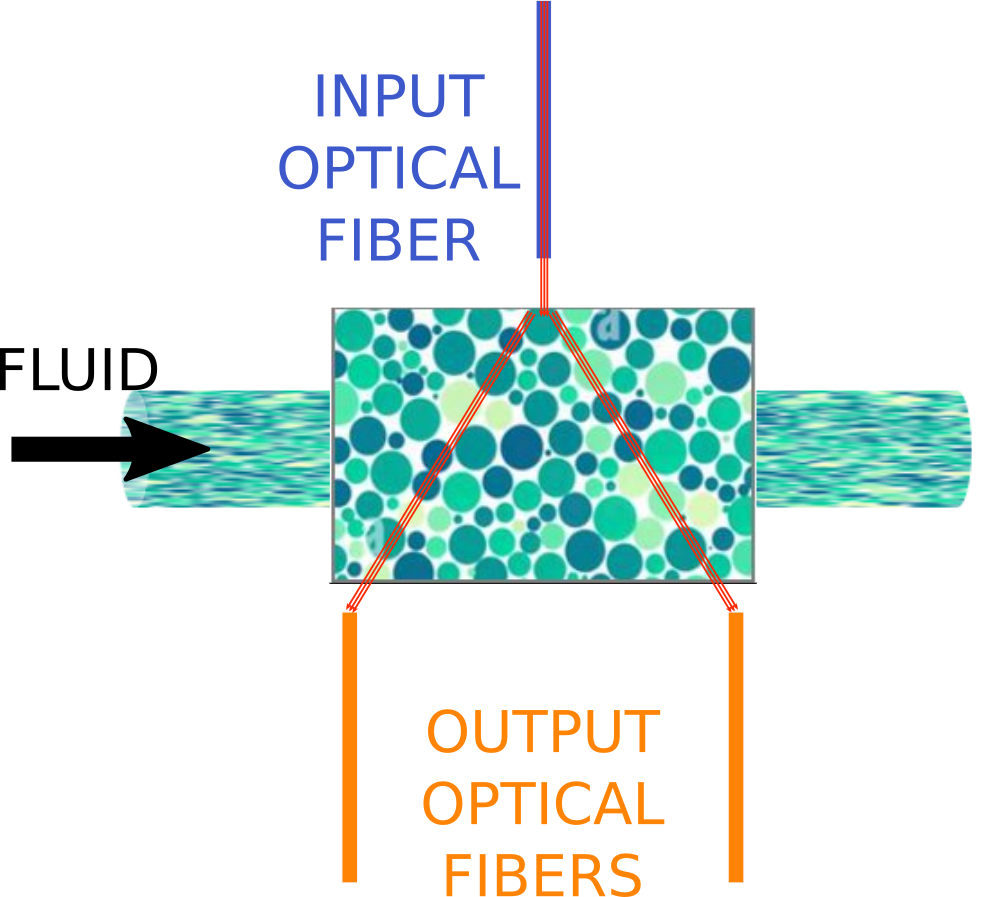
\includegraphics[width=\textwidth]{wp-chamber.png}
		\caption{}
		\label{fig:wp-chamber}
	\end{subfigure}
	\centering
	\begin{subfigure}[b]{0.32\columnwidth}
		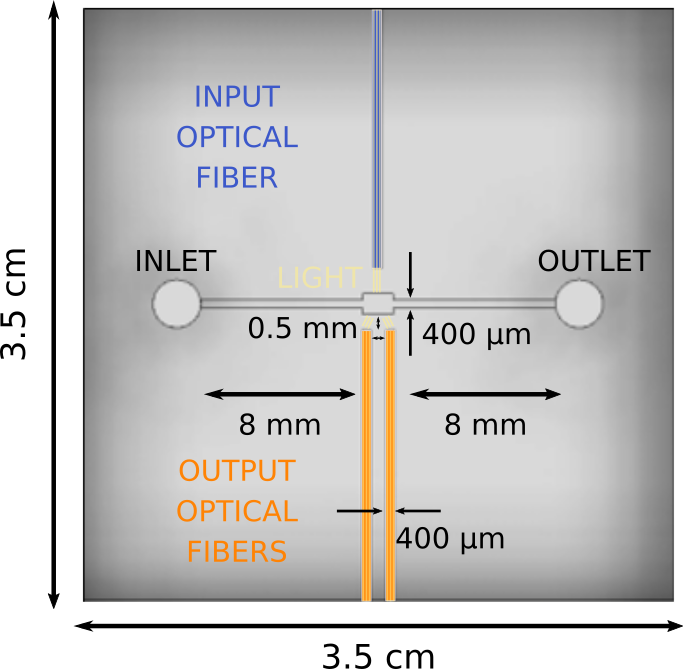
\includegraphics[width=\textwidth]{cad-general.png}
		\caption{}
		\label{fig:cad-chamber}
	\end{subfigure}	
	\begin{subfigure}[b]{0.32\columnwidth}			
		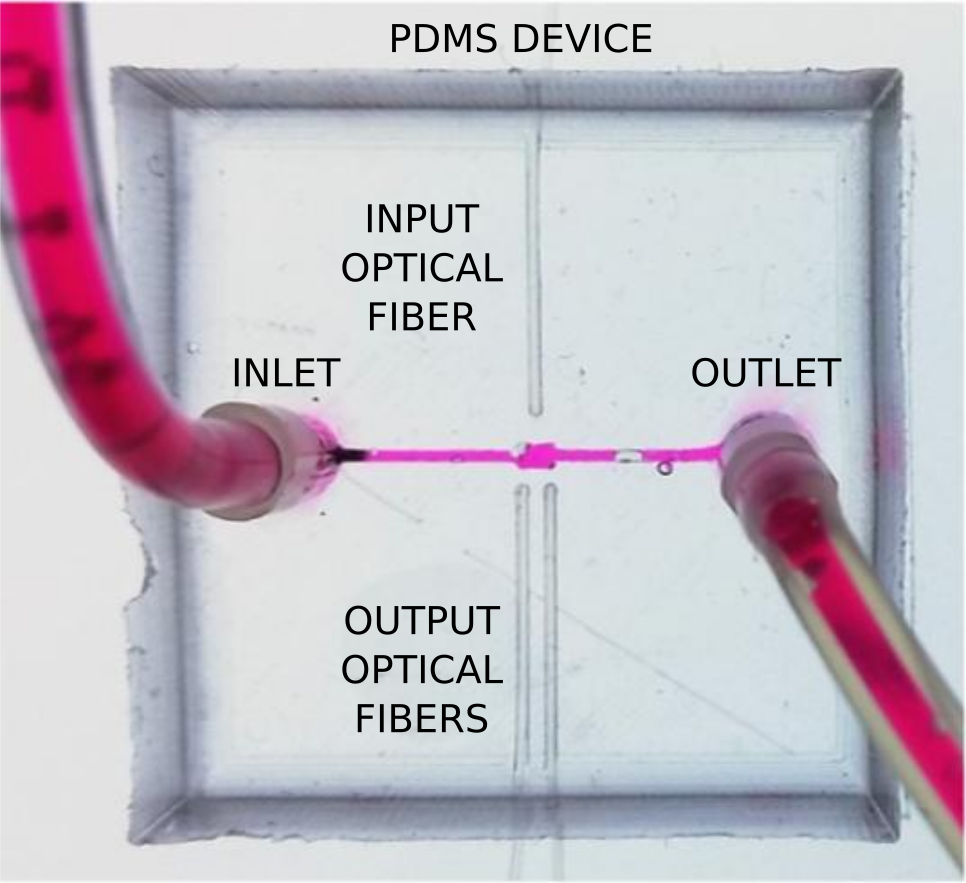
\includegraphics[width=\textwidth]{cad-chamber.png}
		\caption{}
		\label{fig:real-device}
	\end{subfigure}
	\caption{(\ref{fig:wp-chamber}) Working principle of the presented micro-optofludic device; (\ref{fig:cad-chamber}) Frontal view of the CAD representation and its associated dimensions; (\ref{fig:real-device}) A picture depicting the real device. }
\end{figure}
\begin{figure}
	\centering
	\begin{subfigure}[b]{0.8\columnwidth}
		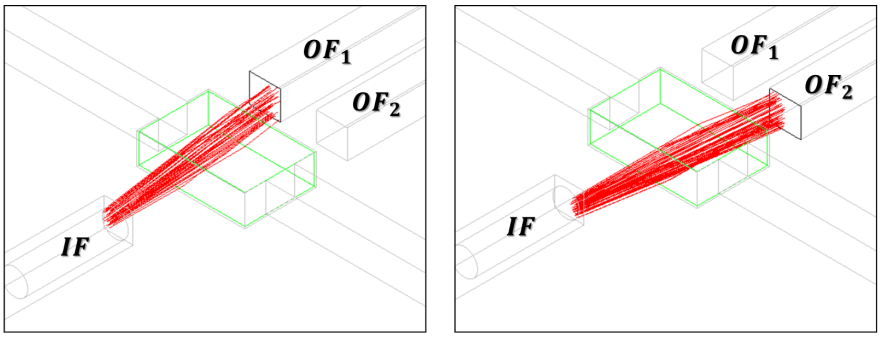
\includegraphics[width=\columnwidth]{d3-rays_path.png}
		\caption{}
		\label{fig:d3-rays_path}
	\end{subfigure}
	\centering
	\begin{subfigure}[b]{0.8\columnwidth}
		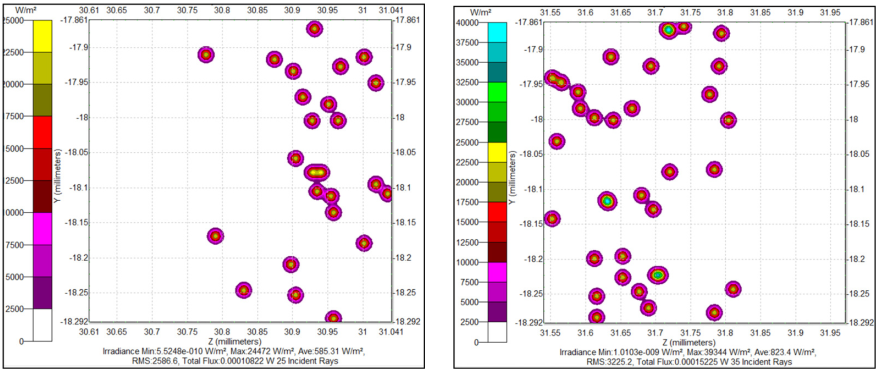
\includegraphics[width=\textwidth]{d1-radiance_map.png}
		\caption{}
		\label{fig:d1-radiance_map}
	\end{subfigure}
	\centering	
	\begin{subfigure}[b]{0.8\columnwidth}			
		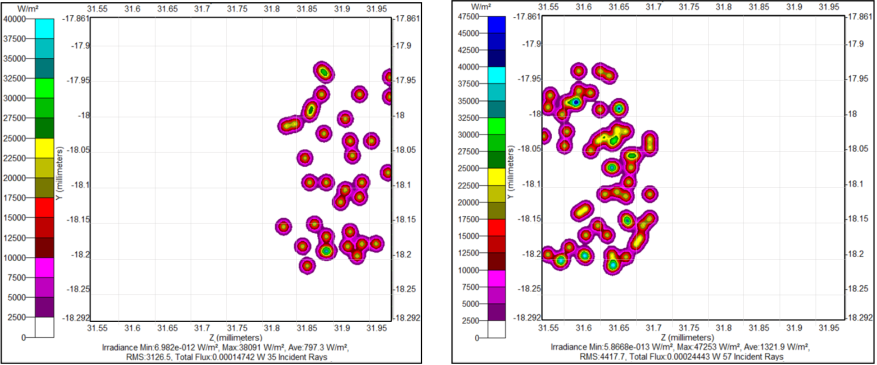
\includegraphics[width=\textwidth]{d2-radiance_map.png}
		\caption{}
		\label{fig:d2-radiance_map}
	\end{subfigure}
	\centering	
	\begin{subfigure}[b]{0.8\columnwidth}			
		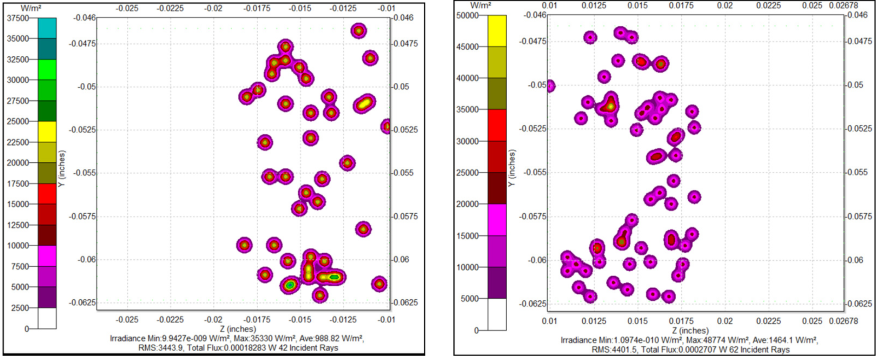
\includegraphics[width=\textwidth]{d3-radiance_map.png}
		\caption{}
		\label{fig:d3-radiance_map}
	\end{subfigure}
	\caption{(\ref{fig:d3-rays_path}) Rays path for \device{3},  (\ref{fig:d1-radiance_map}, \ref{fig:d2-radiance_map}, \ref{fig:d3-radiance_map}) Spatial 2D rays distributions along the section under investigation}
\end{figure}

\section{Working principle and Realization}
In this paper, we present a (PDMS) micro-optofluidic device that uses the light absorption phenomenon to monitor the flow of single-phase or two-phase immiscible fluids. In particular, the aim of the device is to characterize fluids of different types and/or solutions of varying concentrations inside a compartment specifically designed at the core of a microfluidic channel. As shown in \fig\ref{fig:wp-chamber}, \ref{fig:cad-chamber},  \ref{fig:real-device}, the fluid introduced from the inlet, travels through a microchannel 8 $[\rm mm]$ long and 400~$[\rm \mu m]$ wide and is discharged through the outlet. One insertion for the light actuation system and two insertions 400 $[\rm \mu m]$ wide for the optical detecting system constitute the device's micro-optics. Finally, an inter-distance of 0.5. $[\rm mm]$ separates the output optical fibers from one another, and from the device core.


\subsection{Design and Rays Tracing Simulations}
From an operational perspective (see \fig\ref{fig:wp-chamber}), a light beam is generated by the light source produced by the actuation system and directed via the incoming fiber. The beam then travels through the core of the microchip, i.e. the chamber which contains the solution of interest. The outgoing beam is collected by the outgoing fibers and sent to the detecting devices. Due to the fluid's absorption, the exiting light beams will have less intensity than the entering light beam. Such a difference is then used to extrapolate properties of the fluids under investigation.


Given the significance of light in the realization of the aformentioned device, ray tracing simulations have been performed by using TracePro with the aim of determining how different geometrical characteristics can affect the devices' performances. In particular, three distinct devices, results of the different combinations of chamber size, input optical fiber insertion ($\InF$) width $\widthIF$ and inter-distance $\inputInterDistance$ between the chamber and the input optical fiber insertion, depicted as devices \device{1}, \device{2}, \device{3} have been evaluated while keeping constant the microchannel dimensions, the output optical fiber insertions width and the inter-distance $\outputInterDistance$ between the device chamber and the output optical fiber insertion. 
\tab\ref{tab: devices-dimensions} summarizes the dimensions of the three prototypes, while \fig\ref{fig:cad-devices} shows their CAD frontal view together with their dimensions where the most significant changes to each device are highlighted.

\begin{table}[t]
	\centering
	\begin{tabular}{|l|l|c|c|}
		\hline
		& \multicolumn{1}{c|}{\begin{tabular}[c]{@{}c@{}}Chamber\\ Dimensions\end{tabular}} & \begin{tabular}[c]{@{}c@{}}Fiber Insertion\\ Width ($\widthIF$) \end{tabular} & \begin{tabular}[c]{@{}c@{}}Optical Fiber \\ Distance ($\inputInterDistance$)\end{tabular} \\ \hline
		D-1 & 1{[}mm{]} $\times$ 1{[}mm{]} $\times$ 1{[}mm{]}                                   & 1 {[}mm{]}                                                      & 0.5 {[}mm{]}                                                      \\ \hline
		D-2 & 1{[}mm{]} $\times$ 1.5{[}mm{]} $\times$ 0.4{[}mm{]}                               & 0.4 {[}mm{]}                                                    & 0.5 {[}mm{]}                                                      \\ \hline
		D-3 & 1{[}mm{]} $\times$ 1.5{[}mm{]} $\times$ 0.4{[}mm{]}                               & 0.4 {[}mm{]}                                                    & 1 {[}mm{]}                                                        \\ \hline
	\end{tabular}
	
	\caption{Dimensions of the prototypes \device{1}, \device{2}, \device{3}. }
	\label{tab: devices-dimensions}
\end{table}


Simulations consisted in introducing 200 rays at a power $\power=$~1~$[\rm mW]$ into the input optical fiber of each device assuming the chamber was filled with water. 
By looking at the rays path for \device{3}, the light rays radiance 2D maps for each device, shown in \fig\ref{fig:d3-rays_path}, \ref{fig:d1-radiance_map}, \ref{fig:d2-radiance_map}, \ref{fig:d3-radiance_map}, the larger $\inputInterDistance$ and the lower $\widthIF$ , the more incoming rays are perceived by the output optical fiber and the more evenly distributed are along the output optical fiber surface. To be noted, the area between the two output optical fibers is where the majority of the incoming rays concentrate. Although this implied that $\outputInterDistance$ needed to be reduced to improve the incidence rate, further reduction of such a distance was not possible due to limitations in the printing phase. 

A further evidence of the better performances of \device{3} with respect to  \device{1} and  \device{2} is provided by the bar plot shown in \fig\ref{fig:barplot-incidence} where the number of incident rays is significantly higher for \device{3} in both output optical fiber, i.e. left $\OF{1}$ and right one $\OF{2}$. 

\begin{figure}		
	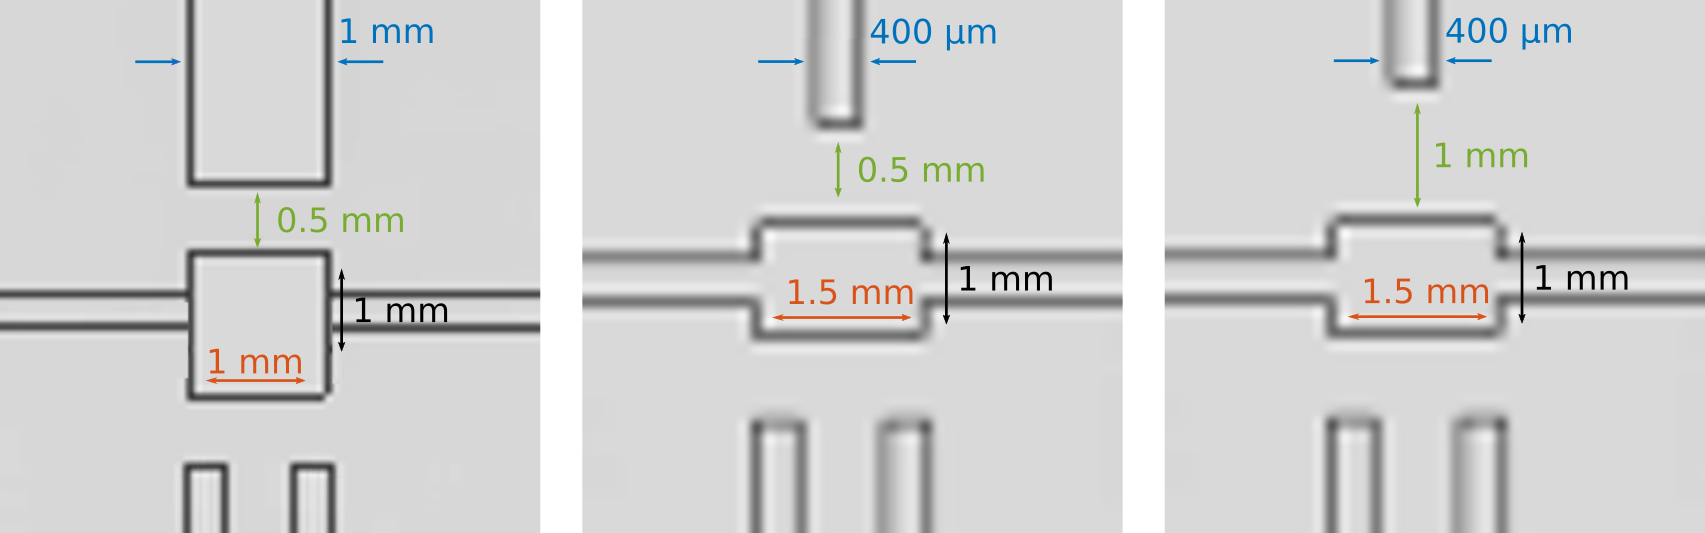
\includegraphics[width=\textwidth, height=0.3\linewidth]{cad-devices.png}
	\caption{\red{remake pictures, resizing to have a rectangular area similar to the current one, add blue highlights of the differences between devices}}
	\label{fig:cad-devices}
\end{figure}

\subsection{Device Realization}

The micro-optofluidic device is realised in PDMS employing a master-slave approach based on inkjet 3D printing technologies. 
The realization consists of several essential steps. First of all, the device's mold is designed and 3D printed with the filaments Ultimaker PLA – M0751 Red for the base and the Ultimaker White Breakway as a \red{support material}. The latter allows to obtain high-quality printed surfaces particularly suitable for the subsequent removal of devices without the need for any further surface post-treatment.
After this stage, the master surfaces go through an ultraviolet (UV) treatment at 35~$^{\circ}[\rm C]$ for 1 hour. 
Then, the PDMS is thoroughly mixed with its curing agent (10:1 ratio), degassed in a desiccator, then poured over the master mold at room temperature for 48 hours. The finished PDMS device is finally separated from the master and bound with a bulk of 0.5 $[\rm mm]$ thickness using a reversible bounding procedure.


\begin{figure}
	\includegraphics[width=\columnwidth]{bar_plots.pdf}
	\caption{Number of incident rays on the surface of interest water passage}
	\label{fig:barplot-incidence}
\end{figure}


\section{Device Characterization}
In this section, we detail the micro-optofluidic device's abilities for distinguishing between various fluids and solutions, as well as their respective concentrations.

\subsection{Experimental Setup}
\usetikzlibrary{calc,fit, positioning}


\begin{figure}[t]
	\centering
\begin{adjustbox}{width=\columnwidth}
\begin{tikzpicture}[
%square node outer loop
squarednodeo/.style={rectangle, draw=white!28, fill=white!25, very thick, minimum size=2mm},
%square node intermediate loop
squarednodei/.style={rectangle, draw=red!35, fill=red!25, very thick, minimum size=8mm},
%square node inner loop
squarednodeii/.style={rectangle, draw=orange!25, fill=orange!20, very thick, minimum size=12mm},
dot/.style={circle, fill=black,	minimum size=1mm, inner sep=0mm, outer sep=0mm,
	node contents={}
},
squarednodefc/.style={rectangle, draw=gray!60, fill=gray!5, very thick, minimum size=12mm},
dot/.style={circle, fill=black,	minimum size=1mm, inner sep=0mm, outer sep=0mm,
	node contents={}
},
squarednodemux/.style={rectangle, draw=black, fill=black, very thick, minimum width=0.5mm, minimum height=30mm},
]
\node (start) [draw=none,fill=none] {};
\node[squarednodefc] (pp) [right=of start]{\shortstack{Syringe Pumps}};
\node[squarednodefc] (hl) [below=of pp]{\shortstack{Halogen Light}};

\node[squarednodefc,outer sep=0pt,right=2.5cm of $(pp)!.5!(hl)$](mc){\shortstack{Microfluidic \\ Chip}};

\node[squarednodefc] (sp) [right=4.5cm of pp]{\shortstack{Spectophotometer}};
\node[squarednodefc] (pd) [right=4.5cm of hl]{\shortstack{Photo Detector}};

\node[squarednodefc,outer sep=0pt,right=2.5cm of $(sp)!.5!(pd)$](pc){\shortstack{PC}};

\draw[- stealth] (pp.east) |- ++ (0.4,0) |- ([yshift= 10pt]mc.west);
\draw[- stealth] (hl.east) |- ++ (0.4,0) |- ([yshift= -10pt]mc.west);

\draw[- stealth] ([yshift= 10pt]mc.east) |- ++ (0.4,0) |- (sp.west);
\draw[- stealth] ([yshift= -10pt]mc.east) |- ++ (0.4,0) |- (pd.west);

\draw[- stealth] (sp.east) |- ++ (0.4,0) |- ([yshift= 10pt]pc.west);
\draw[- stealth] (pd.east) |- ++ (0.4,0) |- ([yshift= -10pt]pc.west);


%\node[squarednodei] (IMU) [right=of start]{IMU};
%\node[squarednodei] (Mocap) [below=3mm of IMU]{Mocap};

%\node (temp)[draw=none,fill=none, above=1mm of IMU] {};
%\node[squarednodei] (VO) [above=3mm of IMU]{VO};
%\node[squarednodei] (GPS) [above=3mm of VO]{GPS};
%\node[squarednodemux] (mux) [right= 30mm of temp] {};p
%\node[squarednodeii] (use) [right=of mux]{\shortstack{Unconstrained \\ State Estimation}};
%\node[squarednodeo] (cse) [right=of use]{\shortstack{Constrained\\State Estimation}};

%\draw [- stealth] (use.east) -- (cse);
%\draw [- stealth] (cse.east) -- (ctrl);
%\draw [- stealth] (mux) -- (use);

% Switch IMU
%\node (isw) [dot, right=of IMU]{};
%\draw (IMU.east) -- (isw.west);
%\node (osw) [dot, right=2mm of isw]{};
%\draw(3.1,0)-- +(-25:0.3);
%\draw[- stealth] (osw.north) |- ++ (0,0) |- ([yshift=-11pt]mux.west);

% Switch Mocap
%\node (isw1) [dot, right=of Mocap]{};
%\draw (Mocap.east) -- (isw1.west);
%\node (osw1) [dot, right=2mm of isw1]{};
%\draw(3.24,-1.11)-- +(-25:0.3);
%\draw[- stealth] (osw1.north) |- ++ (0,0) |- ([yshift=-32pt]mux.west);

% Switch VO
%\node (isw2) [dot, right=of VO]{};
%\draw (VO.east) -- (isw2.west);
%\node (osw2) [dot, right=2mm of isw2]{};
%\draw(3.08,1.14)-- +(-25:0.3);
%\draw[- stealth] (osw2.east) |- ++ (0.3,0) |- ([yshift=12pt]mux.west);

% Switch IMU
%\node (isw3) [dot, right=of GPS]{};
%\draw (GPS.east) -- (isw3.west);
%\node (osw3) [dot, right=2mm of isw3]{};
%\draw(3.1,2.28)-- +(-25:0.3);
%\draw [- stealth] (osw3.east) |- ++ (0.3,0) |- ([yshift=33pt]mux.west);

% Labels
%\put (70, 68) {$\tilde{\vect{p}}$};
%\put (70, 36) {$\tilde{\vect{p}},\tilde{\vect{v}}$};
%\put (70,2) {$\tilde{\vect{a}},\tilde{\vect{\omega}}$};
%\put (70, -30) {$\tilde{\vect{p}}$};

%\put (150, 22) {$\measR{i}$};
%\put (253, 22) {$\stateRest{i}$};
%\put (355, 22) {$\stateRproj{i}$};

\end{tikzpicture}
 \end{adjustbox}
\caption{The complete block diagram of the experimental setup used for the device microptofluidic characterization }
\label{fig:block-diagram}
\end{figure}

% Hardware Setup
A continuous single-phase flow is produced by pumping fluids and solutions of various types and concentrations to the micro optofluidic system's input. \fig\ref{fig:block-diagram} and \fig \ref{fig:exp-setup} show both the block diagram of the experimental setup and the experimental setup used to perform the device characterization. In particular, the fluids and the micro-particles have been pumped by means of a syringe pump (neMESYS) into the opto-microfluidic device at a constant flow rate of $0.1~[\rm ml/min]$. A LED source has been used under the chip for its illumination while an halogen light has been introduced through the input optical fiber and used to illuminate the micro-particles which flow within the microfluidic channel. Light beams that have been changed by the fluids and micro-particles are recovered by the output optical fibers and are then measured by a spectrophotometer (Picoscope) and a photo detector. Such sensors transmit their data to a PC which stores the readings.


\begin{figure}
	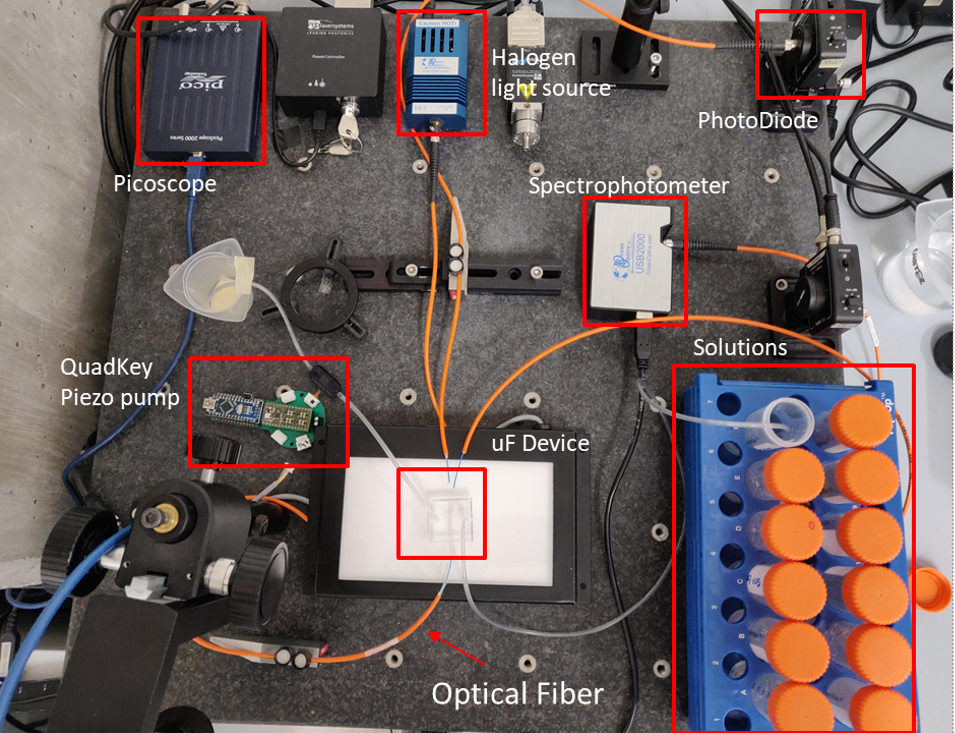
\includegraphics[width=\columnwidth]{exp-setup.png}
	\caption{}
	\label{fig:exp-setup}
\end{figure}

% Experimental Campaigns
\subsection{Experimental Results}
% Results
%% a. Hydrodynamic study for fluids and particles suspension
%% b. Hydrodynamic study for cells and DNA suspension

\section{Conclusions}



\section*{Declarations}

Some journals require declarations to be submitted in a standardised format. Please check the Instructions for Authors of the journal to which you are submitting to see if you need to complete this section. If yes, your manuscript must contain the following sections under the heading `Declarations':

\begin{itemize}
\item Funding
\item Conflict of interest/Competing interests (check journal-specific guidelines for which heading to use)
\item Ethics approval 
\item Consent to participate
\item Consent for publication
\item Availability of data and materials
\item Code availability 
\item Authors' contributions
\end{itemize}

\noindent
If any of the sections are not relevant to your manuscript, please include the heading and write `Not applicable' for that section. 

%%===================================================%%
%% For presentation purpose, we have included        %%
%% \bigskip command. please ignore this.             %%
%%===================================================%%
\bigskip
\begin{flushleft}%
Editorial Policies for:

\bigskip\noindent
Springer journals and proceedings: \url{https://www.springer.com/gp/editorial-policies}

\bigskip\noindent
Nature Portfolio journals: \url{https://www.nature.com/nature-research/editorial-policies}

\bigskip\noindent
\textit{Scientific Reports}: \url{https://www.nature.com/srep/journal-policies/editorial-policies}

\bigskip\noindent
BMC journals: \url{https://www.biomedcentral.com/getpublished/editorial-policies}
\end{flushleft}

\bibliography{bibCustom}% common bib file
\bibliographystyle{sn-basic}
\end{document}
